\chapterimage{./Pictures/cover-gear} % Chapter heading image
\chapter{TP5+TP6 : Hiérarchie de processus, signaux}
\textit{Dans ce TP, nous allons revenir sur quelques commandes en shell pour illustrer le fonctionnement de manière simple, puis nous déporterons ces concepts au travers d’appels systèmes dans une fonction C.}

\section{Gestion des signaux : envoi et reception}
\textit{Les exercices de cette question se concentrent sur les mécanismes d’envoi et de reception des signaux. Ils visent prioritairement à comprendre comment on envoie un signal, quelles sont les conditions nécessaires pour qu’un processus accepte de recevoir un signal, et comment dérouter l’exécution normale d’un programme lorsque ce dernier reçoit un signal. Nous montrons notamment que le concept d’envoi et réception de signaux s’applique aussi bien pour des scripts shell que pour des programmes écrits dans un langage de programmation, ici le C. Dans la section d’après, nous verrons comment ces signaux sont utilisés pour gérer les processus, notamment les phases d’exécution et d’arrêt prématuré.}

\subsection{Exercice 1 : Droits et signaux}
\textit{Cet exercice à pour objectif de nous faire comprendre la nation de droits associés aux signaux. Pour cela, nous utiliserons plusieurs commandes shell, notamment la commande \mintinline{shell}{ps} qui permet de lister les processus actifs sur une machine, et la commande \mintinline{shell}{kill} qui permet d’envoyer un signal à un processus identifié par son pid.}

La commande \mintinline{shell}{kill -l} nous permet de lister l'ensemble des signaux. Pour pouvoir les compter nous éxecutons la commande \mintinline{shell}{kill -l | wc -w} qui compte 31 signaux sur ma machine. On peut envoyer un signal à un processus dont on connait son \texttt{PID} à l'aide de la commande \mintinline{shell}{kill -<SIG_NAME> <PID>}. Par exempler nous pouvons tuer le processus 1285 à l'aide de la commande \mintinline{shell}{kill -SIGKILL 1285}.

Nous écrivons un programme permettant de boucler à l'infinie à l'aide d'une boucle \mintinline{cpp}{while(1)}. Le programme était en \texttt{BASH} je l'ai implémenté en C :
\inputminted[linenos]{cpp}{../sources/cpp/TP5-6/ex1.c}

En éxecutans ce programme dans et en récupérant son PID, nous pouvons dans un terminal, en utilisant la commande \mintinline{shell}{kill} envoyer un signal SIGKILL à ce processus et ainsi mettre fin au programme en le tuant. Si j'envoie le signal à un processus dont je ne suis pas le propriétaire ( appartenant à autre utilisateur ou au root), l'erreur "Operation not authorized" s'affiche. Je peut le vérifier en éxécutant la commande sur un processus root et en vérificant son éxécution dans la liste des processus à l'aide de la commande \mintinline{shell}{top}.

\subsection{Exercice 2 : capture de signal et traduction en langage C}
\textit{Cet exercice nous apprendra capturer des signaux, c’est à dire que l’on peut détecter la réception d’un signal envoyé par un autre processus, et redéfinir le comportement à adopter, c’est à dire la suite d’instructions à exécuter, lorsqu’un signal est détecté.}

J'ai écrit un script shell comportant une boucle infinie affichant un "." chqaue seconde. Le script capture aussi le signal \texttt{SIGINT} et \texttt{SIGUSR1} ainsi si l'utilisateur appuie sur \texttt{CTRL+C} ou envoie un signal \texttt{SIGUSR1} pendant son éxécution un message sera affiché. Ce script lancé ne pourra donc pas être arrété si l'utilisateur appuie sur \texttt{CTRL+C} ou utilise la commande \mintinline{shell}{killl -SIGKILL <PID>}.
Le script et le suivant :
\inputminted{bash}{../sources/cpp/TP5-6/ex2-boucle.sh}
Et maintenant en langage \texttt{C} :
\inputminted[linenos,firstline=5, lastline=27]{cpp}{../sources/cpp/TP5-6/ex2.c}

\subsection{Exercice 3 : Capture de signaux et redirections (exercice difficile)}
\textit{Cet exercice permet de capturés des signaux et les redirigés, c’est à dire que lorsque le signal est reçu, on redéfinit le comportement par défaut qu’aurait du avoir le processus. Dans un premier temps, nous allons voir quel est le comportement par défaut des processus lors de la réception d’un signal. Dans un  second temps, nous allons redéfinir le comportement d’un processus à la réception d’un signal.}

Plusieurs signaux permettent de terminer l'exécution d'un porocessus. Afin de pouvoir savoir lesquels nous allons écrire un script. Pour chaque signal X, un processus sera lancé en arrière plan, ici le script de la boucle infinie sera utilisé. Son PID sera retrouvé grace à la variable \mintinline{bash}{$!} afin de lui envoyer le signal X. À l'aide de la commande \mintinline{shell}{ps -p <PID>} nous saurons si le processus à été arrété, ainsi on pourra conclure que le signal X tuje ou pas le processus.
Voici le script :
\inputminted[linenos]{bash}{../sources/cpp/TP5-6/ex3-testKillerSignal.sh}

\subsection{Exercice 4 : envoi multiples et capture de signal en C}
\textit{Au terme des exercices précédents nous avons compris les notions de signal, de redirection et de mise en oeuvre en langage shell. L'objectif de cet exercice est la simple traduction de ce qui a été vu en shell en langage C, et l’étude d’une autre commande nommée killall}
Nous avons besoin dans un premier temps du code ayant une boucle infinie et capturant le signal SIGINT (CTRL+C). Le script est ci-dessous :
\inputminted{bash}{../sources/cpp/TP5-6/ex4-captureShell.sh}
Et maintenant en langage \texttt{C} :
\inputminted[linenos,firstline=5, lastline=23]{cpp}{../sources/cpp/TP5-6/ex4.c}
Nous pouvons maintenant lancer 3 processus de notre programme C afin de les tuers avec la commande \mintinline{shell}{killall -SIGINT ex4}.
On essaie aussi de les mettre en pause et des les relancer grace aux commandes
\begin{itemize}
\item \mintinline{shell}{killall -SIGSTOP ex4}
\item \mintinline{shell}{killall -SIGCONT ex4}
\end{itemize}
Puis nous les tuons grace à la commande \mintinline{shell}{killall -9 ex4}

\section{Gestion des processus}

\subsection{Exercice 5 : Processus en premier-plan / Arriere-plan}
\textit{Nous allons voir ici comment manipuler les processus pour les passer tantôt en premier-plan, tantôt en arrière-plan, les stopper et les relancer. Ces manipulations sont rendues possibles par l’utilisation de signaux, et les fonctionnalités de deux programmes : bg (background) et fg (foreground)}
La commande \mintinline{shell}{ps aux} permet d'afficher l'etat d'execution des processus.
Il affiche le status du processus :
\begin{itemize}
\item R : "runnable", veut dire que le processus est prêt à être éxécuté.
\item S : "sleeping", veut dire que le processus est endormi.
\item D : veut dire que le processus est sommeil interruptible.
\item T : "traced", veut dire que le processus est arrété ou suivi.
\item Z : zombie
\end{itemize}
Le \texttt{+} qui suit indique si le processus est en arrière plan.

%\subsection{Exercice 6 : Duplication et recouvrement de processus}
%\textit{Dans cet exercice, nous recouvrons un processus existant, d’abord au travers d’un script shell, puis en appliquant ce concept au sein d’un programme C.}

\section{Gestion des processus - Suite}

\subsection{Exercice 7 : Duplication de processus}
\textit{L’objectif de cet exercice est de comprendre la notion de processus parent et de processus enfant lors de la duplication d’un processus par l’appel à la fonction \mintinline{shell}{fork()}. Nous y revoyons la notion de PID et PPID (ou PID du parent) vus en cours. L’objectif est de mettre en évidence le role de l’appel à l’instruction fork() ainsi que la particularité de son code retour, et d’identifier que lors d’une duplication, le processus nouvellement créé ne reprend pas au début de son code mais poursuit l’exécution du processus parent. On rappelle que \mintinline{shell}{fork()} retourne 0 dans le processus nouvellement créé (fils) et une valeur strictement supérieure à 0 sinon (qui correspond au PID du processus nouvellement créé)}

\subsection{Exercice 8 : Creation et destruction de processus}
\textit{Cet exercice rappelle les notions de processus zombie et processus orphelin, et définit les modalités d’apparition de ces deux types particuliers de processus.}
En lançant la commande \mintinline{shell}{ps -aux} on peut observer le statut des processus.

\paragraph{1. Processus zombie}
Un processus zombie est un processus présent alors que sont processus parent ayant terminé son exécution, il reste présent sur le système, en attente d'être pris en compte par son processus parent..

\paragraph{2. Processus orphelin}
Un processus orphelin est un processus présent alors que sont processus parent est mort. Le processus orphelin est donc "adopté" par le processus 1, le processus "init"

\subsection{Exercice 9 : Evaluation du nombre de processus}
\textit{L’objectif de cet exercice est de comprendre le résultat de l’appel à l’instruction \mintinline{shell}{fork()} ainsi que la particularité de son code retour, et d’identifier que lors d’une duplication, le processus nouvellement créé ne reprend pas au début de son code mais poursuit l’exécution du processus parent. On rappelle que \mintinline{cpp}{fork()} retourne 0 dans le processus nouvellement créé (fils) et une valeur strictement supérieure à 0 sinon (qui correspond au PID du processus nouvellement créé).}

\paragraph{1. premier programme :}
\inputminted[linenos,firstline=5, lastline=9]{cpp}{../sources/cpp/TP5-6/ex9-programme1.c}
Nous pouvons expliquer le code ci-dessus par le schema suivant :
\begin{figure}[H]
\centering
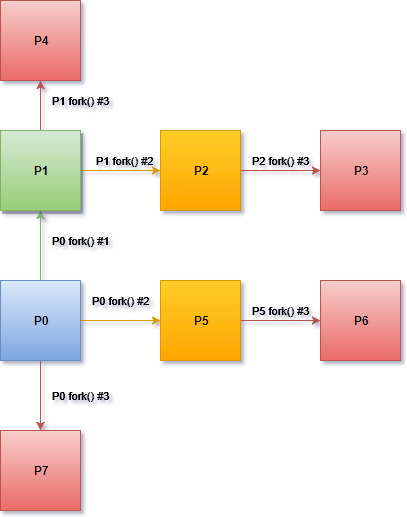
\includegraphics[width=200pt]{./cpp/Pictures/tp5+tp6-ex9-programme1}
\caption{Duplication de processus 1}
\label{Duplication de processus 1}
\end{figure}

\paragraph{2. deuxième programme :}
\inputminted[linenos,firstline=5, lastline=9]{cpp}{../sources/cpp/TP5-6/ex9-programme2.c}
Nous pouvons expliquer le code ci-dessus par le schema suivant :
\begin{figure}[H]
\centering
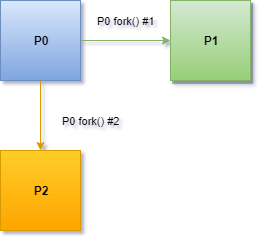
\includegraphics[width=200pt]{./cpp/Pictures/tp5+tp6-ex9-programme2}
\caption{Duplication de processus 2}
\label{Duplication de processus 2}
\end{figure}

\paragraph{3. troisieme programme :}
\inputminted[linenos,firstline=5, lastline=13]{cpp}{../sources/cpp/TP5-6/ex9-programme3.c}
Nous pouvons expliquer le code ci-dessus par le schema suivant :
\begin{figure}[H]
\centering
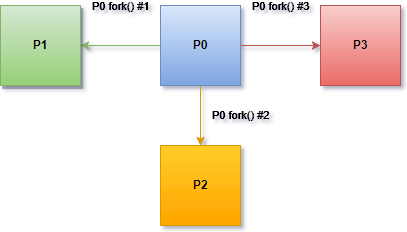
\includegraphics[width=200pt]{./cpp/Pictures/tp5+tp6-ex9-programme3}
\caption{Duplication de processus 3}
\label{Duplication de processus 3}
\end{figure}

\subsection{Exercice 10 : Conjonctions, Disjonctions, et Duplication}
\textit{L’objectif de cet exercice est de comprendre le résultat de l’appel à l’instruction \mintinline{cpp}{fork()} ainsi que la particularité de son code retour, et d’identifier que lors d’une duplication, le processus nouvellement créé ne reprend pas au début de son code mais poursuit l’exécution du processus parent.}

En éxécutant quelques programmes exemple ci-dessous nous pouvons déterminer le fonctionnement des conjonctions et des disjonctions.

\paragraph{1. premier programme :}
\inputminted[linenos,firstline=5, lastline=8]{cpp}{../sources/cpp/TP5-6/ex10-conjonction1.c}
\begin{enumerate}
\item Le processus père P0 : éxécute le premer \mintinline{cpp}{fork()} créant le processus P1 et retourne une valeur non-nulle et s'arrete.
\item Le processus fils P1 : la valeur du premier \mintinline{cpp}{fork()} est égale à 0 et évalue \mintinline{cpp}{&&}
\item Le processus fils P1 : éxécute donc le deuxième \mintinline{cpp}{fork()} fork créant P2 ainsi que le troisieme \mintinline{cpp}{fork()} créant P3
\item Le processus fils P2 : la valeur du deuxième \mintinline{cpp}{fork()} retourne 0, cour-circuite \mintinline{cpp}{&&} et s'arrete.
\item Le processus fils P3 : la valeur du troisième \mintinline{cpp}{fork()} retourne 0 et s'arrete.
\end{enumerate}

Nous pouvons expliquer le code ci-dessus par le schema suivant :
\begin{figure}[H]
\centering
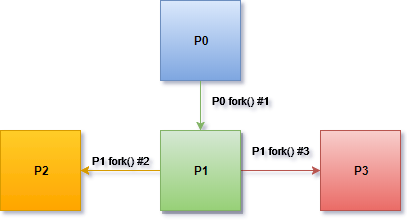
\includegraphics[width=200pt]{./cpp/Pictures/tp5+tp6-ex10-conjonction1}
\caption{Conjonction de processus 1}
\label{Conjonction de processus 1}
\end{figure}

\paragraph{2. deuxième programme :}
\inputminted[linenos,firstline=5, lastline=8]{cpp}{../sources/cpp/TP5-6/ex10-conjonction2.c}
\begin{enumerate}
\item Le processus père P0 éxécute le premier \mintinline{cpp}{fork()} créant le processus P1 et retourne une valeur non-nulle.
\item Le processus fils P1 la valeur du premier \mintinline{cpp}{fork()} est égale à 0 et court-circuite \mintinline{cpp}{&&} et s'arrete.
\item Le processus père P0 : la valeur du premier \mintinline{cpp}{fork()} est non-nulle et évalue \mintinline{cpp}{||} et effectue le deuxième \mintinline{cpp}{fork}.
\item Le processus fils P2 : la valeur du deuxième \mintinline{cpp}{fork()} retourne 0 et exécute donc le troisieme \mintinline{cpp}{fork()} créant P3.
\item Le processus fils P2 s'arrete.
\item Le processus fils P3 s'arrete.
\end{enumerate}
Nous pouvons expliquer le code ci-dessus par le schema suivant :
\begin{figure}[H]
\centering
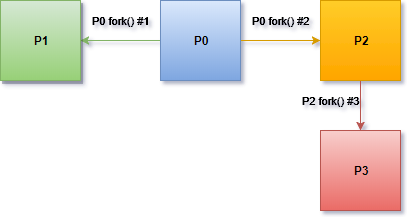
\includegraphics[width=200pt]{./cpp/Pictures/tp5+tp6-ex10-conjonction2}
\caption{Conjonction de processus 2}
\label{Conjonction de processus 2}
\end{figure}

\subsection{Exercice 11 : Terminaison normale de processus}
\textit{L’objectif de cet exercice est de placer correctement les instructions \mintinline{cpp}{wait()}}

Lorsque le processus fils se termine avant le processus père, il devient un zombie. Pour permettre à un processus fils en état zombie de disparaître complètement, on utilise la \mintinline{cpp}{wait()}.

\paragraph{1. premier programme :}
\inputminted[linenos,firstline=5, lastline=11]{cpp}{../sources/cpp/TP5-6/ex11-programme1.c}

\paragraph{2. deuxième programme :}
\inputminted[linenos,firstline=5, lastline=14]{cpp}{../sources/cpp/TP5-6/ex11-programme2.c}

\paragraph{3. troisieme programme :}
\inputminted[linenos,firstline=5, lastline=19]{cpp}{../sources/cpp/TP5-6/ex11-programme3.c}
